\documentclass[a4paper,12pt]{ltjsarticle}

% LuaLaTeX用パッケージ
\usepackage{luatexja}
\usepackage{luatexja-fontspec}
\usepackage{amsmath, amssymb, amsthm}
\usepackage{mathtools}
\usepackage{tikz}
\usepackage{tikz-cd}
\usepackage[margin=2.5cm]{geometry}
\usepackage{hyperref}
\usepackage{enumitem}
\usepackage{tcolorbox}
\tcbuselibrary{theorems,skins,breakable}

% TikZライブラリ
\usetikzlibrary{arrows.meta, positioning, decorations.pathreplacing, calc, shapes.geometric, patterns, shadows}

% 定理環境
\theoremstyle{definition}
\newtheorem{theorem}{定理}[section]
\newtheorem{lemma}[theorem]{補題}
\newtheorem{proposition}[theorem]{命題}
\newtheorem{definition}[theorem]{定義}
\newtheorem{example}[theorem]{例}
\newtheorem{remark}[theorem]{注意}
\newtheorem{corollary}[theorem]{系}

% カスタムボックス
\newtcolorbox{maintheorem}[1][]{
  colback=blue!5!white,
  colframe=blue!75!black,
  fonttitle=\bfseries,
  title=#1,
  breakable
}

\newtcolorbox{keyidea}[1][]{
  colback=green!5!white,
  colframe=green!75!black,
  fonttitle=\bfseries,
  title=#1,
  breakable
}

\newtcolorbox{bourbaki}[1][]{
  colback=purple!5!white,
  colframe=purple!75!black,
  fonttitle=\bfseries,
  title=#1,
  breakable
}

\newtcolorbox{historical}[1][]{
  colback=orange!5!white,
  colframe=orange!75!black,
  fonttitle=\bfseries,
  title=#1,
  breakable
}

% コマンド定義
\newcommand{\N}{\mathbb{N}}
\newcommand{\R}{\mathbb{R}}
\newcommand{\Z}{\mathbb{Z}}
\newcommand{\cat}[1]{\mathbf{#1}}
\newcommand{\Hom}{\mathrm{Hom}}
\newcommand{\id}{\mathrm{id}}
\DeclareMathOperator{\Ob}{Ob}

\title{構造塔の圏論的形式化\\
  {\large CAT2\_complete.lean: ブルバキの構造理論と圏論}\\
  {\large 学部生向け数学解説}}
\author{Claude Code により生成\\
  {\small Lean 4 コード: Codex (OpenAI)}\\
  {\small \TeX 解説: Claude Code}\\
  {\small プロジェクト: \texttt{lean-natural-numbers}}}
\date{\today}

\begin{document}

\maketitle

\begin{abstract}
本稿では、ニコラ・ブルバキの『数学原論』における構造理論（Theory of Structures）を圏論的に形式化した構造塔（Structure Tower）について解説する。構造塔は集合に階層的な構造を与える数学的概念であり、各要素が属する「最小の層」を持つことで、射の一意性と普遍性が保証される。本解説は学部3-4年生を対象とし、圏論の基礎知識を前提とする。Lean 4による完全な形式化を通じて、現代的な数学基礎論の視点からブルバキの思想を再考する。
\end{abstract}

\tableofcontents

\section{序論：ブルバキと構造の数学}

\subsection{歴史的背景}

\begin{historical}[ニコラ・ブルバキとは]
ニコラ・ブルバキ（Nicolas Bourbaki）は、1930年代にフランスの数学者グループが創設した集団ペンネームである。彼らの主著『数学原論』（Éléments de mathématique）は、数学全体を公理的・構造的観点から再構築する壮大なプロジェクトであった。

特に重要なのが\textbf{構造理論}（Theory of Structures）であり、これは集合に代数構造、順序構造、位相構造などを統一的に扱う枠組みを提供する。
\end{historical}

\subsection{構造塔の動機}

数学において、同じ集合に異なる「レベル」の構造を与えることがしばしばある：

\begin{example}[実数の階層構造]
実数 $\R$ には以下のような階層構造が存在する：
\begin{itemize}
\item \textbf{層0}：有理数 $\mathbb{Q}$
\item \textbf{層1}：代数的数（多項式方程式の解）
\item \textbf{層2}：すべての実数 $\R$
\end{itemize}
各層は前の層を含み、より「豊かな」構造を持つ。
\end{example}

\begin{center}
\begin{tikzpicture}[scale=1.2]
  % 層の描画（同心円的に）
  \draw[fill=blue!10, draw=blue!50, very thick] (0,0) ellipse (1 and 0.6);
  \node at (0,0) {$\mathbb{Q}$};
  \node[blue!70!black, left] at (-1.2,0) {層0};

  \draw[fill=green!10, draw=green!50, very thick] (0,0) ellipse (2 and 1.2);
  \node[green!70!black, right] at (2.2,0) {層1: 代数的数};

  \draw[fill=red!10, draw=red!50, very thick] (0,0) ellipse (3 and 1.8);
  \node[red!70!black, right] at (3.2,0) {層2: $\R$};

  % 包含関係の矢印
  \draw[-Stealth, thick] (0,-2.3) -- (0,-2.8) node[midway, right] {包含};
\end{tikzpicture}
\end{center}

\subsection{本稿の目的}

本稿では、構造塔の以下の側面を解説する：

\begin{enumerate}
\item \textbf{定義}：構造塔の公理的定義と\texttt{minLayer}の役割
\item \textbf{圏構造}：構造塔が圏をなすこと
\item \textbf{普遍性}：自由構造塔の普遍性
\item \textbf{積構造}：直積と射影の普遍性
\item \textbf{形式化}：Lean 4による厳密な実装
\end{enumerate}

\section{構造塔の定義}

\subsection{基本概念}

\begin{definition}[最小層を持つ構造塔]\label{def:structure_tower}
\textbf{最小層を持つ構造塔}（Structure Tower with Minimal Layer）とは、以下のデータの組 $(X, I, \leq, (X_i)_{i \in I}, \mathrm{minLayer})$ である：

\begin{enumerate}
\item $X$：\textbf{基礎集合}（carrier）
\item $I$：\textbf{添字集合}で、半順序 $\leq$ を持つ
\item $(X_i)_{i \in I}$：各 $i \in I$ に対する $X$ の部分集合の族（\textbf{層}）
\item \textbf{被覆性}（covering）：$\bigcup_{i \in I} X_i = X$
\item \textbf{単調性}（monotonicity）：$i \leq j \Rightarrow X_i \subseteq X_j$
\item $\mathrm{minLayer} : X \to I$：各 $x \in X$ に対して、$x$ を含む\textbf{最小の層}を選ぶ関数
\item \textbf{最小性}：
  \begin{itemize}
  \item $x \in X_{\mathrm{minLayer}(x)}$（$\mathrm{minLayer}(x)$ は実際に $x$ を含む）
  \item $x \in X_i \Rightarrow \mathrm{minLayer}(x) \leq i$（最小であることの保証）
  \end{itemize}
\end{enumerate}
\end{definition}

\begin{center}
\begin{tikzpicture}[scale=1.3]
  % 添字集合 I の図
  \node at (-4,3) {\textbf{添字集合 $I$}};
  \foreach \i/\y in {0/0, 1/1, 2/2, 3/3} {
    \node[circle, draw, fill=gray!20] (i\i) at (-4,\y) {$i_{\i}$};
  }
  \draw[-Stealth] (i0) -- (i1) node[midway, right] {$\leq$};
  \draw[-Stealth] (i1) -- (i2);
  \draw[-Stealth] (i2) -- (i3);

  % 基礎集合 X とその層
  \node at (2,3.5) {\textbf{基礎集合 $X$ と層 $X_i$}};

  % 層の描画
  \foreach \i/\y/\col in {0/0/blue, 1/1/green, 2/2/orange, 3/3/red} {
    \draw[fill=\col!20, draw=\col!70, very thick, rounded corners]
      (-0.5,\y-0.3) rectangle (4.5,\y+0.3);
    \node[\col!70!black, left] at (-0.7,\y) {$X_{i_{\i}}$};
  }

  % 要素の配置
  \node[circle, fill=blue!70, inner sep=2pt] (x1) at (0.5,0) {};
  \node[below] at (x1) {$x_1$};

  \node[circle, fill=green!70, inner sep=2pt] (x2) at (1.5,1) {};
  \node[above] at (x2) {$x_2$};

  \node[circle, fill=orange!70, inner sep=2pt] (x3) at (2.5,2) {};
  \node[above] at (x3) {$x_3$};

  \node[circle, fill=red!70, inner sep=2pt] (x4) at (3.5,3) {};
  \node[above] at (x4) {$x_4$};

  % minLayer の対応
  \draw[-Stealth, dashed, thick] (x1) to[bend right] node[midway, below left] {\tiny $\mathrm{minLayer}$} (i0);
  \draw[-Stealth, dashed, thick] (x2) to[bend right] (i1);
  \draw[-Stealth, dashed, thick] (x3) to[bend right] (i2);
  \draw[-Stealth, dashed, thick] (x4) to[bend right] (i3);

  % 包含関係の注釈
  \draw[decorate, decoration={brace, amplitude=5pt, mirror}]
    (4.7,0) -- (4.7,3) node[midway, right=5pt] {\small 単調性: $X_i \subseteq X_j$};
\end{tikzpicture}
\end{center}

\subsection{minLayerの重要性}

\begin{keyidea}[minLayerがなぜ必要か]
構造塔において、各要素は複数の層に属しうる（単調性より）。しかし、射を一意に定義するためには、「どの層に本質的に属するか」を決める必要がある。

\textbf{minLayer}はこの曖昧性を解消する：
\begin{itemize}
\item 各 $x \in X$ に対して、$x$ が属する最小の層 $\mathrm{minLayer}(x)$ を選ぶ
\item 射 $f : X \to Y$ は、$\mathrm{minLayer}(f(x)) = \varphi(\mathrm{minLayer}(x))$ を満たす必要がある
\item これにより、添字写像 $\varphi : I \to J$ が一意に決定される
\end{itemize}
\end{keyidea}

\begin{bourbaki}[ブルバキの精神：構造の保存]
ブルバキにおいて、数学的構造を扱う射は「構造を保存する」写像である。構造塔の射は：
\begin{enumerate}
\item 基礎集合の写像 $f : X \to Y$
\item 添字集合の順序保存写像 $\varphi : I \to J$
\item \textbf{重要}：$\varphi(\mathrm{minLayer}_X(x)) = \mathrm{minLayer}_Y(f(x))$
\end{enumerate}
この第3条件（\texttt{minLayer\_preserving}）が、普遍性の一意性を保証する鍵である。
\end{bourbaki}

\section{構造塔の圏構造}

\subsection{射の定義}

\begin{definition}[構造塔の射]\label{def:hom}
構造塔 $T = (X, I, (X_i), \mathrm{minLayer}_X)$ から $T' = (Y, J, (Y_j), \mathrm{minLayer}_Y)$ への\textbf{射}は、対 $(f, \varphi)$ であって：

\begin{enumerate}
\item $f : X \to Y$（基礎集合の写像）
\item $\varphi : I \to J$（添字集合の順序保存写像）
\item \textbf{層構造の保存}：$x \in X_i \Rightarrow f(x) \in Y_{\varphi(i)}$
\item \textbf{minLayerの保存}：$\mathrm{minLayer}_Y(f(x)) = \varphi(\mathrm{minLayer}_X(x))$
\end{enumerate}
\end{definition}

\begin{center}
\begin{tikzpicture}[scale=1.0]
  % 左側：構造塔 T
  \node at (-3,4) {\textbf{構造塔 $T$}};
  \draw[fill=blue!10, rounded corners] (-4.5,0) rectangle (-1.5,3);
  \node at (-3,2.5) {$X$};
  \draw[thick] (-4.3,0.5) -- (-1.7,0.5) node[midway, below] {$X_i$};
  \node[circle, fill=red, inner sep=2pt] (x) at (-3,1.5) {};
  \node[right] at (x) {$x$};

  \draw[fill=gray!20] (-4,0) rectangle (-3.5,3.5);
  \node at (-3.75,3.7) {$I$};
  \node (i) at (-3.75,0.7) {$i$};

  % 右側：構造塔 T'
  \node at (3,4) {\textbf{構造塔 $T'$}};
  \draw[fill=green!10, rounded corners] (1.5,0) rectangle (4.5,3);
  \node at (3,2.5) {$Y$};
  \draw[thick] (1.7,0.8) -- (4.3,0.8) node[midway, below] {$Y_{\varphi(i)}$};
  \node[circle, fill=red, inner sep=2pt] (fx) at (3,1.5) {};
  \node[right] at (fx) {$f(x)$};

  \draw[fill=gray!20] (4.5,0) rectangle (5,3.5);
  \node at (4.75,3.7) {$J$};
  \node (phii) at (4.75,1.0) {$\varphi(i)$};

  % 射の矢印
  \draw[-Stealth, very thick, blue] (x) -- (fx) node[midway, above] {$f$};
  \draw[-Stealth, very thick, purple] (i) -- (phii) node[midway, below] {$\varphi$};

  % minLayer の矢印
  \draw[-Stealth, dashed, red] (x) to[bend left] node[near start, left] {\tiny $\mathrm{minLayer}_X$} (-3.75,1.5);
  \draw[-Stealth, dashed, red] (fx) to[bend right] node[near start, right] {\tiny $\mathrm{minLayer}_Y$} (4.75,1.5);
\end{tikzpicture}
\end{center}

\subsection{圏の法則}

\begin{theorem}[構造塔の圏]\label{thm:category}
構造塔は圏 $\cat{StructureTower}$ をなす：
\begin{enumerate}
\item \textbf{対象}：最小層を持つ構造塔
\item \textbf{射}：定義\ref{def:hom}の射
\item \textbf{恒等射}：$\id_T = (\id_X, \id_I)$
\item \textbf{合成}：$(g, \psi) \circ (f, \varphi) = (g \circ f, \psi \circ \varphi)$
\end{enumerate}
圏の法則（結合律、単位律）が成り立つ。
\end{theorem}

\begin{proof}[証明の概略]
\textbf{結合律}：
\[
((h, \chi) \circ (g, \psi)) \circ (f, \varphi) = (h \circ g \circ f, \chi \circ \psi \circ \varphi) = (h, \chi) \circ ((g, \psi) \circ (f, \varphi))
\]

\textbf{単位律}：
\[
(g, \psi) \circ (\id_X, \id_I) = (g \circ \id_X, \psi \circ \id_I) = (g, \psi)
\]
\[
(\id_Y, \id_J) \circ (f, \varphi) = (\id_Y \circ f, \id_J \circ \varphi) = (f, \varphi)
\]

\textbf{minLayer\_preserving の保存}：
\begin{align*}
\mathrm{minLayer}_{T''}((g \circ f)(x))
&= \mathrm{minLayer}_{T''}(g(f(x))) \\
&= \psi(\mathrm{minLayer}_{T'}(f(x))) \quad (\text{$g$ のminLayer保存}) \\
&= \psi(\varphi(\mathrm{minLayer}_T(x))) \quad (\text{$f$ のminLayer保存}) \\
&= (\psi \circ \varphi)(\mathrm{minLayer}_T(x))
\end{align*}
\end{proof}

\begin{center}
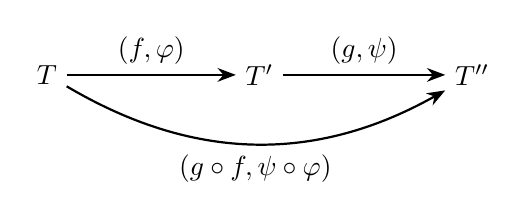
\begin{tikzpicture}[scale=0.9]
  % 合成の可換図式
  \node (T) at (0,0) {$T$};
  \node (T') at (3,0) {$T'$};
  \node (T'') at (6,0) {$T''$};

  \draw[-Stealth, thick] (T) -- (T') node[midway, above] {$(f, \varphi)$};
  \draw[-Stealth, thick] (T') -- (T'') node[midway, above] {$(g, \psi)$};
  \draw[-Stealth, thick, bend right=30] (T) to node[midway, below] {$(g \circ f, \psi \circ \varphi)$} (T'');
\end{tikzpicture}
\end{center}

\section{自由構造塔と普遍性}

\subsection{自由構造塔の構成}

\begin{definition}[自由構造塔]\label{def:free_tower}
半順序集合 $X$ から生成される\textbf{自由構造塔} $\mathcal{F}(X)$ を次のように定義する：
\begin{itemize}
\item 基礎集合：$X$ そのもの
\item 添字集合：$I = X$（同じ半順序）
\item 層：$X_i = \{x \in X \mid x \leq i\}$（下集合）
\item minLayer：$\mathrm{minLayer}(x) = x$（自分自身）
\end{itemize}
\end{definition}

\begin{example}[自然数の自由構造塔]
$X = \N$（通常の順序）とすると：
\begin{itemize}
\item $X_0 = \{0\}$
\item $X_1 = \{0, 1\}$
\item $X_2 = \{0, 1, 2\}$
\item $\mathrm{minLayer}(n) = n$
\end{itemize}
\end{example}

\begin{center}
\begin{tikzpicture}[scale=1.1]
  \node at (0,4) {\textbf{自然数の自由構造塔}};

  % 層の描画
  \foreach \n in {0,1,2,3} {
    \draw[fill=blue!20, draw=blue!60, very thick, rounded corners]
      (0,\n*0.8) rectangle (2+\n*0.5,\n*0.8+0.5);
    \node[blue!70!black] at (-0.7,\n*0.8+0.25) {$X_{\n}$};

    % 要素の配置
    \foreach \k in {0,...,\n} {
      \node[circle, fill=red!70, inner sep=1.5pt] at (0.3+\k*0.5,\n*0.8+0.25) {};
    }
  }

  \draw[decorate, decoration={brace, amplitude=5pt}]
    (-1.2,0) -- (-1.2,2.9) node[midway, left=5pt] {\small 包含: $X_i \subseteq X_j$};
\end{tikzpicture}
\end{center}

\subsection{普遍性}

\begin{maintheorem}[自由構造塔の普遍性]\label{thm:universal}
半順序集合 $X$ と構造塔 $T$ に対して、任意の単調写像 $f : X \to T.\mathrm{carrier}$ であって
\[
x \leq y \Rightarrow \mathrm{minLayer}_T(f(x)) \leq \mathrm{minLayer}_T(f(y))
\]
を満たすものに対して、\textbf{一意的な}射 $\Phi : \mathcal{F}(X) \to T$ が存在して
\[
\Phi.\mathrm{map}(x) = f(x) \quad \text{for all } x \in X
\]
が成り立つ。
\end{maintheorem}

\begin{keyidea}[普遍性の一意性の鍵]
定理\ref{thm:universal}の一意性は、\texttt{minLayer\_preserving}条件から導かれる：

任意の射 $\Psi : \mathcal{F}(X) \to T$ で $\Psi.\mathrm{map} = f$ を満たすものに対して、
\begin{align*}
\Psi.\mathrm{indexMap}(x)
&= \Psi.\mathrm{indexMap}(\mathrm{minLayer}_{\mathcal{F}(X)}(x)) \\
&= \mathrm{minLayer}_T(\Psi.\mathrm{map}(x)) \quad (\text{minLayer保存}) \\
&= \mathrm{minLayer}_T(f(x))
\end{align*}
したがって、$\Psi.\mathrm{indexMap}$ は完全に決定される。
\end{keyidea}

\begin{proof}[定理\ref{thm:universal}の証明]
\textbf{存在性}：射 $\Phi = (\Phi.\mathrm{map}, \Phi.\mathrm{indexMap})$ を次のように構成：
\begin{itemize}
\item $\Phi.\mathrm{map}(x) := f(x)$
\item $\Phi.\mathrm{indexMap}(x) := \mathrm{minLayer}_T(f(x))$
\end{itemize}

\textbf{順序保存性の確認}：
$x \leq y$ ならば、仮定より $\mathrm{minLayer}_T(f(x)) \leq \mathrm{minLayer}_T(f(y))$。

\textbf{層構造の保存}：
$x \in X_i$（すなわち $x \leq i$）とする。このとき
\begin{align*}
\Phi.\mathrm{map}(x) &= f(x) \\
\mathrm{minLayer}_T(f(x)) &\leq \mathrm{minLayer}_T(f(i)) = \Phi.\mathrm{indexMap}(i)
\end{align*}
単調性より $f(x) \in T_{\Phi.\mathrm{indexMap}(i)}$。

\textbf{minLayer保存}：
\begin{align*}
\mathrm{minLayer}_T(\Phi.\mathrm{map}(x))
&= \mathrm{minLayer}_T(f(x)) \\
&= \Phi.\mathrm{indexMap}(x) \\
&= \Phi.\mathrm{indexMap}(\mathrm{minLayer}_{\mathcal{F}(X)}(x))
\end{align*}

\textbf{一意性}：Key Ideaで示した通り。
\end{proof}

\begin{center}
\begin{tikzpicture}[scale=1.0]
  % 普遍性の図式
  \node (X) at (0,2) {$X$};
  \node (FX) at (0,0) {$\mathcal{F}(X)$};
  \node (T) at (4,0) {$T$};

  \draw[-Stealth, thick, dashed] (X) -- (T) node[midway, above] {$f$（単調写像）};
  \draw[-Stealth, thick] (FX) -- (X) node[midway, left] {\small 包含};
  \draw[-Stealth, thick, red] (FX) -- (T) node[midway, below] {$\exists! \Phi$};

  \node at (2,1.5) {\textcolor{red}{一意的な射}};
\end{tikzpicture}
\end{center}

\section{直積と射影}

\subsection{直積の構成}

\begin{definition}[構造塔の直積]\label{def:product}
二つの構造塔 $T_1, T_2$ の\textbf{直積} $T_1 \times T_2$ を次のように定義：
\begin{itemize}
\item 基礎集合：$X_1 \times X_2$
\item 添字集合：$I_1 \times I_2$（積順序）
\item 層：$(X_1 \times X_2)_{(i,j)} = X_1^{(i)} \times X_2^{(j)}$
\item minLayer：$\mathrm{minLayer}((x, y)) = (\mathrm{minLayer}_1(x), \mathrm{minLayer}_2(y))$
\end{itemize}
\end{definition}

\begin{center}
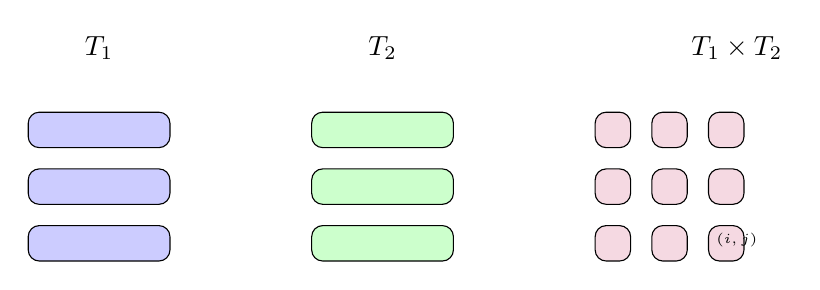
\begin{tikzpicture}[scale=0.9]
  % T1 の層
  \node at (-3,3) {\textbf{$T_1$}};
  \foreach \i in {0,1,2} {
    \draw[fill=blue!20, rounded corners] (-4,\i*0.8) rectangle (-2,\i*0.8+0.5);
  }

  % T2 の層
  \node at (1,3) {\textbf{$T_2$}};
  \foreach \j in {0,1,2} {
    \draw[fill=green!20, rounded corners] (0,\j*0.8) rectangle (2,\j*0.8+0.5);
  }

  % T1 × T2 の層（格子状）
  \node at (6,3) {\textbf{$T_1 \times T_2$}};
  \foreach \i in {0,1,2} {
    \foreach \j in {0,1,2} {
      \draw[fill=purple!15, rounded corners]
        (4+\i*0.8,\j*0.8) rectangle (4.5+\i*0.8,\j*0.8+0.5);
    }
  }

  \node at (6,0.3) {\tiny $(i,j)$};
\end{tikzpicture}
\end{center}

\subsection{積の普遍性}

\begin{theorem}[積の普遍性]\label{thm:product_universal}
構造塔 $T, T_1, T_2$ と射 $f_1 : T \to T_1$, $f_2 : T \to T_2$ に対して、\textbf{一意的な}射
\[
\Phi : T \to T_1 \times T_2
\]
が存在して、次の図式が可換になる：
\[
\begin{tikzcd}
T \arrow[dr, "\exists! \Phi", dashed] \arrow[ddr, "f_1"', bend right] \arrow[drr, "f_2", bend left] & & \\
& T_1 \times T_2 \arrow[d, "\pi_1"] \arrow[r, "\pi_2"] & T_2 \\
& T_1 &
\end{tikzcd}
\]
すなわち、$\Phi \circ \pi_1 = f_1$ かつ $\Phi \circ \pi_2 = f_2$。
\end{theorem}

\begin{proof}[証明の概略]
\textbf{存在性}：
\[
\Phi.\mathrm{map}(x) := (f_1.\mathrm{map}(x), f_2.\mathrm{map}(x))
\]
\[
\Phi.\mathrm{indexMap}(i) := (f_1.\mathrm{indexMap}(i), f_2.\mathrm{indexMap}(i))
\]

\textbf{minLayer保存}：
\begin{align*}
\mathrm{minLayer}_{T_1 \times T_2}(\Phi.\mathrm{map}(x))
&= (\mathrm{minLayer}_{T_1}(f_1.\mathrm{map}(x)), \mathrm{minLayer}_{T_2}(f_2.\mathrm{map}(x))) \\
&= (f_1.\mathrm{indexMap}(\mathrm{minLayer}_T(x)), f_2.\mathrm{indexMap}(\mathrm{minLayer}_T(x))) \\
&= \Phi.\mathrm{indexMap}(\mathrm{minLayer}_T(x))
\end{align*}

\textbf{一意性}：任意の射 $\Psi : T \to T_1 \times T_2$ で可換性を満たすものに対して、射影との可換性とminLayer保存から $\Psi = \Phi$ が導かれる。
\end{proof}

\section{具体例と応用}

\subsection{自然数の構造塔}

\begin{example}[自然数による実装]
\begin{verbatim}
def natTowerMin : StructureTowerWithMin where
  carrier := ℕ
  Index := ℕ
  layer := fun n => {k : ℕ | k ≤ n}
  minLayer := id
\end{verbatim}

この構造塔では：
\begin{itemize}
\item 各自然数 $n$ が最小層 $X_n = \{0, 1, \ldots, n\}$ を定義
\item $\mathrm{minLayer}(k) = k$（自分自身が最小層）
\item 後者関数 $\mathrm{succ} : \N \to \N$ が誘導する射が一意に存在
\end{itemize}
\end{example}

\subsection{同型射}

\begin{definition}[同型射]
構造塔の\textbf{同型射} $f : T \xrightarrow{\sim} T'$ とは、射 $f : T \to T'$ と $g : T' \to T$ の対であって
\[
g \circ f = \id_T, \quad f \circ g = \id_{T'}
\]
を満たすものである。
\end{definition}

\begin{proposition}[同型射での全単射性]
$f : T \xrightarrow{\sim} T'$ が同型射ならば、基礎写像 $f.\mathrm{map} : X \to Y$ は全単射である。
\end{proposition}

\section{忘却関手と圏論的視点}

\subsection{忘却関手}

構造塔の圏から他の圏への自然な関手が存在する：

\begin{definition}[忘却関手]
\begin{enumerate}
\item \textbf{基礎集合への忘却}：
\[
U_{\mathrm{carrier}} : \cat{StructureTower} \to \cat{Type}
\]
各構造塔 $T$ をその基礎集合 $T.\mathrm{carrier}$ に対応させる。

\item \textbf{添字集合への忘却}：
\[
U_{\mathrm{Index}} : \cat{StructureTower} \to \cat{Type}
\]
各構造塔 $T$ をその添字集合 $T.\mathrm{Index}$ に対応させる。
\end{enumerate}
\end{definition}

\begin{center}
\begin{tikzpicture}[scale=1.0]
  % 圏の図式
  \node (ST) at (0,2) {$\cat{StructureTower}$};
  \node (Type1) at (-3,0) {$\cat{Type}$};
  \node (Type2) at (3,0) {$\cat{Type}$};

  \draw[-Stealth, thick] (ST) -- (Type1) node[midway, left] {$U_{\mathrm{carrier}}$};
  \draw[-Stealth, thick] (ST) -- (Type2) node[midway, right] {$U_{\mathrm{Index}}$};

  \node[rounded corners, draw, fill=yellow!20] at (0,-1) {忘却関手};
\end{tikzpicture}
\end{center}

\subsection{自由-忘却随伴}

自由構造塔の構成 $\mathcal{F}$ と忘却関手 $U_{\mathrm{carrier}}$ の間には、随伴関係が成り立つ（完全な証明は本稿の範囲を超える）：

\[
\Hom_{\cat{StructureTower}}(\mathcal{F}(X), T) \cong \Hom_{\cat{Poset}}(X, U_{\mathrm{carrier}}(T))
\]

\section{まとめ}

\subsection{構造塔の意義}

構造塔は、ブルバキの構造理論を圏論的に形式化したものである。重要なポイント：

\begin{enumerate}
\item \textbf{階層性}：集合に階層的な構造を与える
\item \textbf{最小性}：$\mathrm{minLayer}$ により曖昧性を解消
\item \textbf{普遍性}：自由構造塔の普遍性により、射が一意に決定される
\item \textbf{圏論}：積、射影、忘却関手など、圏論的構造が豊富
\end{enumerate}

\subsection{Lean 4による形式化の意義}

本稿で解説した内容は、Lean 4で完全に形式化されている（\texttt{CAT2\_complete.lean}）：

\begin{tcolorbox}[colback=gray!10, colframe=black, title=Lean 4コードへのリンク]
\texttt{src/MyProjects/ST/CAT2\_complete.lean}

主な定理：
\begin{itemize}
\item 圏構造：119-125行目
\item 普遍性：243-275行目
\item 積の普遍性：323-384行目
\end{itemize}
\end{tcolorbox}

\subsection{今後の展望}

構造塔の理論は、以下の方向に拡張可能である：

\begin{itemize}
\item \textbf{極限と余極限}：より一般的な普遍構成
\item \textbf{随伴関手}：自由-忘却随伴の完全な証明
\item \textbf{モナド構造}：構造塔上のモナドの研究
\item \textbf{高次圏論}：2-圏としての構造塔
\end{itemize}

\section*{参考文献}

\begin{enumerate}
\item Nicolas Bourbaki, \textit{Éléments de mathématique: Théorie des ensembles}
\item Saunders Mac Lane, \textit{Categories for the Working Mathematician}, Springer (1971)
\item The mathlib Community, \textit{The Lean Mathematical Library}, \url{https://github.com/leanprover-community/mathlib4}
\item Corry, Leo, \textit{Modern Algebra and the Rise of Mathematical Structures}, Birkhäuser (2004)
\end{enumerate}

\appendix

\section{Leanコードの詳細}

\subsection{StructureTowerWithMinの定義}

Lean 4での定義（44-63行目）：
\begin{verbatim}
structure StructureTowerWithMin where
  carrier : Type u
  Index : Type v
  [indexPreorder : Preorder Index]
  layer : Index → Set carrier
  covering : ∀ x : carrier, ∃ i : Index, x ∈ layer i
  monotone : ∀ {i j : Index}, i ≤ j → layer i ⊆ layer j
  minLayer : carrier → Index
  minLayer_mem : ∀ x, x ∈ layer (minLayer x)
  minLayer_minimal : ∀ x i, x ∈ layer i → minLayer x ≤ i
\end{verbatim}

各フィールドがブルバキの公理に対応している。

\subsection{圏構造の実装}

圏のインスタンス（119-125行目）：
\begin{verbatim}
instance : CategoryTheory.Category (StructureTowerWithMin.{u, v}) where
  Hom := Hom
  id := Hom.id
  comp := fun f g => Hom.comp g f
  id_comp := by intros; rfl
  comp_id := by intros; rfl
  assoc := by intros; rfl
\end{verbatim}

圏の法則が自明に成り立つことが、定義の良さを示している。

\end{document}
